%
% $Id: ch04_implementation.tex
%
%   *******************************************************************
%   * SEE THE MAIN FILE "AllegThesis.tex" FOR MORE INFORMATION.       *
%   *******************************************************************
%
\chapter{Experimental Results}\label{ch:implem}
Our experiments consisted of having every agent play one another multiple times on different sized boards of each game under different time allowances.  Each pair of agents played games on 5x5, 7x7, 9x9, 11x11, and 13x13 Go as well as 9x9, 11x11, and 14x14 Hex.  For each of these gametypes, 20 games were played with time allowances of 500ms, 1000ms, 2000ms, 4000ms, and 8000ms.  The different board sizes provide different branching factors (e.g. 13x13 Go has a much higher branching factor than 7x7 Go), while the different time allowances allow for each agent to run through more iterations of MCTS on each turn.  In the course of our experiments, we were able to uncover several interesting performance trends.

This chapter is organized by game; there is one section covering the reseults from the Go gameplay, and another on the results from the Hex gameplay.  In each section, we first note the agents' performances against the trivial \texttt{RandomAgent}, then overview the results from each experimental agent's games against \texttt{MCTSAgent}, and then finally look at the head-to-head games between the experimental agents.  Note that due to the size and number of our data visualizations, we will often cite Appendix \ref{appa:data}, which houses all of our data visualizations in full, when referencing data.  While most of the full visualizations will not be in this chapter, some small snippets will be included.  

For some context on the Go score visualizations, consider Figure \ref{fig:ex} as an example.  Each colored line represents the score of a different game of Go, whose size and time allowance is specified at the top of the Figure.  Each line plots the score of a single playout over the course of a 250 move game.  A positive score is a good score for the first player, while a negative score is a good score for the second player --- so here, a positive score is good for \texttt{ANNAgent}, while a negative score is good for \texttt{MCTSAgent}.  The smooth, gray curve shows the overall score across all plays of the game at each move for the given configuration.

\begin{figure}[h]
  \centering
  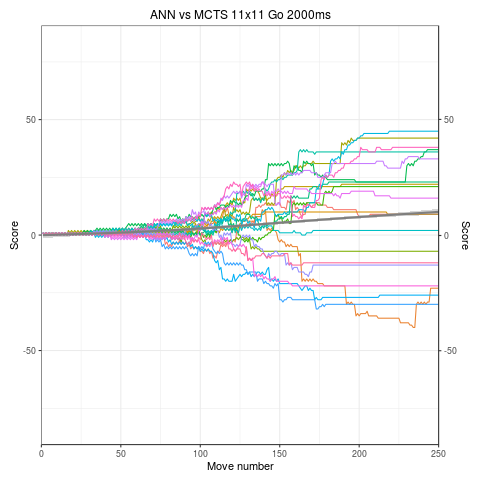
\includegraphics[scale=0.6]{images/Visualizations/ANNvsMCTS/2000ms11x11.png}
  \caption{Example Visualization}
  \label{fig:ex}
\end{figure}
  

\section{Go}
The results of the games between each intelligent agent and the \texttt{RandomAgent} are surprisingly significant.  We assumed each of the intelligent agents would vastly outperform the \texttt{RandomAgent}, and the raw win/loss numbers for these games (Table \ref{tab:ranloss}) seem to indicate exactly this --- each agent won between 98\% and 99\% of their games against the \texttt{RandomAgent}.  However, the plots tracking the game scores over the course of the games tell a different story.  The \texttt{MCTSAgent} and \texttt{ANNAgent} appear to have a normal performance --- they usually take a quick lead and rarely give up points, regardless of board size or time allowance.  This, however, was not the case for the \texttt{GAAgent}.

\begin{table}
\centering
\begin{tabular}{|c|c|c|}
\hline
\textbf{Agent Type} & \textbf{Losses to RandomAgent} & \textbf{Total Games}\\ \hline\hline
\texttt{MCTSAgent} & 5 & 400\\ \hline
\texttt{ANNAgent} & 6 & 400\\ \hline
\texttt{GAAgent} & 7 & 400\\ \hline
\end{tabular}
\caption{Intelligent Agent Losses to \texttt{RandomAgent}}
\label{tab:ranloss}
\end{table}

\begin{figure}[h]
\centering
\begin{minipage}{.45\textwidth}
  \centering
  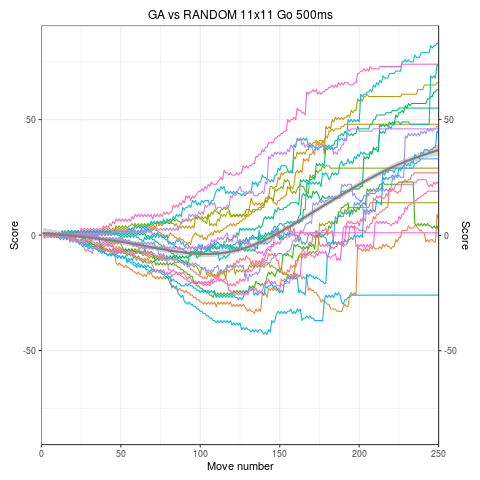
\includegraphics[scale=0.4]{images/Visualizations/GAvsRANDOM/500ms11x11.png}
\end{minipage}%
\begin{minipage}{.45\textwidth}
  \centering
  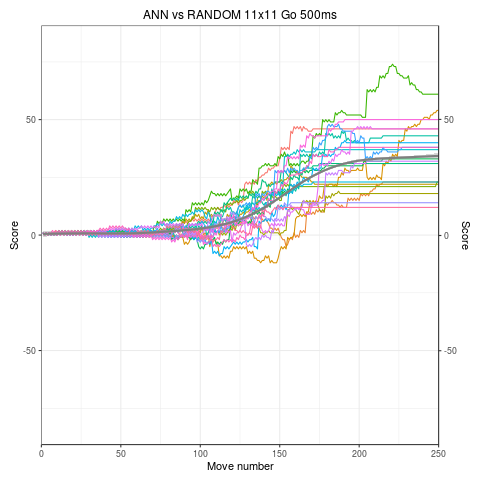
\includegraphics[scale=0.4]{images/Visualizations/ANNvsRANDOM/500ms11x11.png}
\end{minipage}
\caption{\texttt{GAAgent}'s and \texttt{ANNAgent}'s performance against \texttt{RandomAgent}}
\label{fig:rand}
\end{figure}

For large boards and/or a small time allowance, the \texttt{GAAgent} has a tendency to actually fall behind the \texttt{RandomAgent} for a significant portion of the game.  The larger the board and smaller the time allowance, the longer the agent performs poorly; the agent's performance always seems to vastly improve later in the game, though, leading to a seemingly higher performance.  Note the shape of the two graphs in Figure \ref{fig:rand}, which compares the performance of the \texttt{GAAgent} and \texttt{ANNAgent} against the \texttt{RandomAgent}.

The \texttt{GAAgent} only loses a single game of this configuration, even ending with a higher average score than the \texttt{ANNAgent}.  However at turn 150 out of 250, on average the \texttt{GAAgent} is actually losing by a significant amount against the \texttt{RandomAgent}.  Meanwhile the \texttt{ANNAgent} is consistently winning almost all of its games at move 150.  This can be observed happening between other game configurations in Figure \ref{app:garandscore} of Appendix \ref{appa:data}.  This type of performance ended up being a trend for the \texttt{GAAgent}.

\begin{figure}[h]
\centering
\begin{minipage}{.45\textwidth}
  \centering
  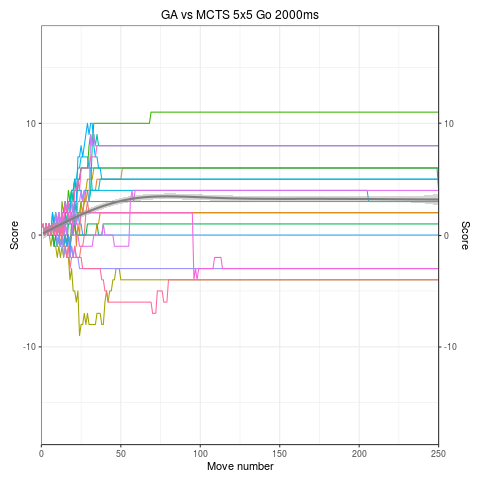
\includegraphics[scale=0.4]{images/Visualizations/GAvsMCTS/2000ms5x5.png}
\end{minipage}%
\begin{minipage}{.45\textwidth}
  \centering
  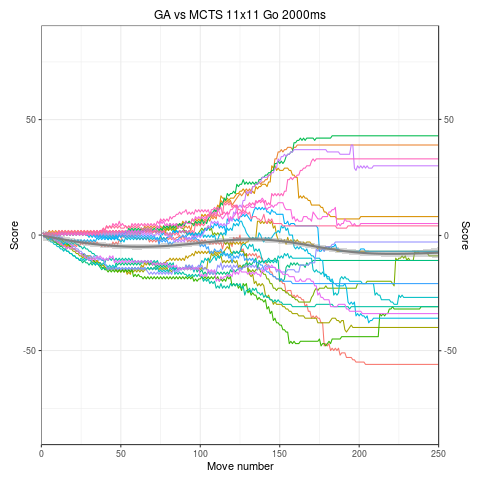
\includegraphics[scale=0.4]{images/Visualizations/GAvsMCTS/2000ms11x11.png}
\end{minipage}
\caption{\texttt{GAAgent} vs \texttt{MCTSAgent} performance on different board sizes}
\label{fig:gamcts}
\end{figure}

The results of the games between \texttt{ANNAgent} and \texttt{MCTSAgent} (Appendix \ref{appa:data} Figure \ref{app:annmctsscore}) are quite conclusive.  The \texttt{ANNAgent} consistently slightly outperforms the \texttt{MCTSAgent} regardless of board size and time allowance.  While the \texttt{MCTSAgent} did manage to win a number of games in each board configuration, we can see that the average score favors the \texttt{ANNAgent} in 18 out of 20 board configurations.  On the two configurations for which the \texttt{ANNAgent} did not outperform the \texttt{MCTSAgent}, the average score was 0, favoring neither agent.

\begin{figure}[h]
\centering
\begin{minipage}{.45\textwidth}
  \centering
  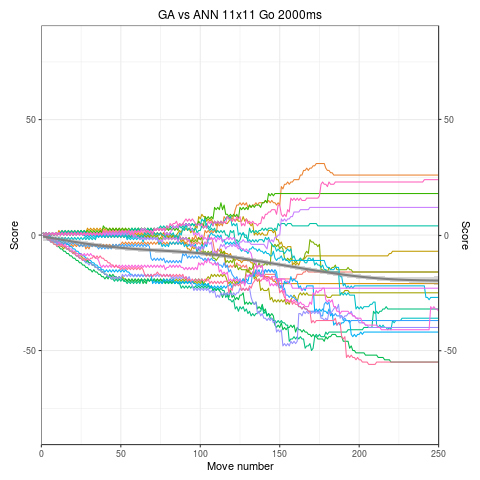
\includegraphics[scale=0.4]{images/Visualizations/GAvsANN/2000ms11x11.png}
\end{minipage}%
\begin{minipage}{.45\textwidth}
  \centering
  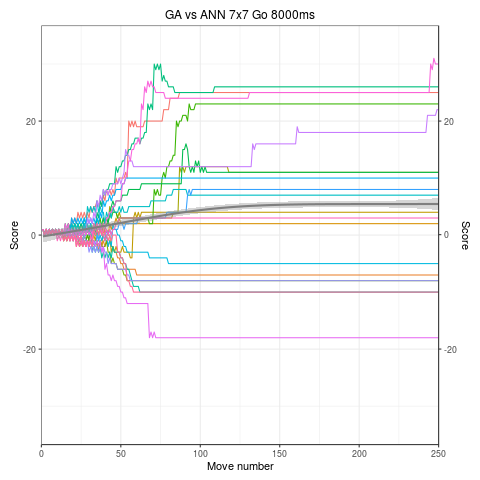
\includegraphics[scale=0.4]{images/Visualizations/GAvsANN/8000ms7x7.png}
\end{minipage}
\caption{\texttt{ANNAgent} and \texttt{GAAgent} on their more dominant board configurations}
\label{fig:gamcts}
\end{figure}

The \texttt{GAAgent}'s results against the \texttt{MCTSAgent} are rather consistent with what was observed against the \texttt{RandomAgent} --- essentially, performance trends upwards as the time allowance increases, and performance trends downwards as board size increases.  An example of this can be seen in Figure \ref{fig:gamcts}, which shows the scores for two board sizes at the same time allowance.  Each row of graphs in Appendix A Figure \ref{appa:gamctsscore} clearly shows this trend --- scores favor \texttt{MCTSAgent} more and more as board size increases.  The \texttt{GAAgent}, though, does tend to outperform the \texttt{MCTSAgent}.  While not as dominant as the \texttt{ANNAgent}, it was able to achieve a higher average score for the majority of board configurations, especially those with smaller boards or higher time allowances.

The head-to-head matchups between \texttt{GAAgent} and \texttt{ANNAgent} provide the most obvious patterns in our data, and further confirms our suspicions about the \texttt{GAAgent}'s performance trend.  The \texttt{GAAgent} was able to achieve a higher average score on every set of games which had either a 5x5 game board (the smallest size used), or a time allowance of 8000ms (the highest time allowance used).  Meanwhile the \texttt{ANNAgent} tended to have a much better performance on boards with a lower time allowance and larger board size, most notably on the 11x11 and 9x9 boards (excluding those with an 8000ms time allowance).

The configurations which had both a moderate board size and moderate time allowance led to the games being somewhat of a tossup between the two agents.  Some configurations saw the \texttt{GAAgent} with the higher average score, while others gave it to the \texttt{ANNAgent}.  In general, the more moderate the board size and time allowance, the closer the average game score tended to 0.

\section{Final Analysis}
The results of the experiments painted a shockingly clear picture.  We found that the \texttt{ANNAgent}'s performance was rather consistent regardless of board size or time allowance. It's tree pruning technique provides a moderate boost in performance over a standard Monte-Carlo Tree Search, and does not noticably change with such changes in board configuration.  This demonstrates the value of having certain nodes in the game tree be visited a higher number of times, even at the expense of a smaller number of overall MCTS iterations.  Because of this, it can be used to reliably improve on MCTS without a need to worry about the structure of the game.

The \texttt{GAAgent} can also provide a demonstrable boost in performance over standard MCTS, but its algorithm's performance is much more dependant on the board size and time allowance it is given.  Its performance has a strong positive correlation with time allowance, and a strong negative correlation with board size.  Overall, this leads its performance to be much more variable.  It can outperform the \texttt{ANNAgent} in some configurations, but in others it can struggle against even the trivial \texttt{RandomAgent}.

We can explain the \texttt{GAAgent}'s performance trend rather easily.  Because of the random starting point of its population of heuristic weights, it requires a large number of iterations through MCTS before its population can find a decent hueristic function.  With a low time allowance or a large board size, it simply cannot find an appropriate heuristic function until rather late in the game.  This does, however, speak to the potential power of this type of agent.  Despite its notably bad performance early on in many games, it was often able to outperform its opponent and win by the end of the game.

The agent, though, is likely very dependant on starting with an appropriate hueristic.  If the things the agent is measuring on the board as its hueristic do not represent a realistic strategy, it is very likely the agent would perform poorly --- its performance may even be lower than a standard MCTS.